% Problem 2 Solution
Let us start with the Navier-Stokes equations for an incompressible fluid.
\begin{align}
    \frac{\partial \vec{u}}{\partial t} + (\vec{u}\cdot\vec{\nabla})\vec{u} &= -\frac{1}{\rho}\vec{\nabla}p + \frac{\mu}{\rho}\nabla^2\vec{u} + \vec{f}\\
    \vec{\nabla}\cdot\vec{u} &= 0
\end{align}
Assuming that the external body forces acting on the fluid are negligible allows us to omit the last term on the right-hand side of the momentum equation.
\begin{equation}
    \frac{\partial \vec{u}}{\partial t} + (\vec{u}\cdot\vec{\nabla})\vec{u} = -\frac{1}{\rho}\vec{\nabla}p + \frac{\mu}{\rho}\nabla^2\vec{u}
    \label{nsm}
\end{equation}
Also, under the steady, fully developed flow assumption, the total time derivative can be taken as zero.
\begin{equation}
    \frac{d\vec{u}}{dt} = \frac{\partial \vec{u}}{\partial t} + (\vec{u}\cdot\vec{\nabla})\vec{u} = 0
\end{equation}
Furthermore, if the pressure gradient is zero, we can drop the first term on the right-hand side of equation (\ref{nsm}), which allows us to write the simplified momentum equation as 
\begin{equation}
    \nu\nabla^2\vec{u} = 0,
\end{equation}
where $\nu = \mu/\rho$ is the kinematic viscosity. Notice that we may rewrite the last equation as 
\begin{equation}
    \nabla^2\vec{u} = 0
\end{equation}
since it is understood that the kinematic viscosity is non-zero. 

Now, we are also told that the flow is two-dimensional, and since it is assumed that the flow does not vary along $x$, we may write $\vec{u} = u(y)\ \hat{x}$. Notice that we have concluded that $u=u(y)$, which allows us to write a single ordinary differential equation for $u(y)$.
\begin{equation}
    \frac{d^2u}{dy^2} = 0
    \label{odeu}
\end{equation}
We can then solve equation (\ref{odeu}) by direct integration to obtain the following solution.
\begin{equation}
    u(y) = c_1 y + c_2
\end{equation}
At this point, we must apply the boundary conditions. Remember that we are working with no-slip boundary conditions, which implies that $u(h)=U$ and $u(-h)=0$.
\begin{align}
    u(-h) &= 0 = -c_1 h + c_2 \label{bct}\\
    u(h) &= U = c_1 h + c_2 \label{bcb}
\end{align}
Solving equations (\ref{bct}) and (\ref{bcb}) simultaneously for $c_1$ and $c_2$ yields $c_1 = U/2h$ and $c_2 = U/2$. Thus, the velocity field for this particular geometry is
\begin{equation}
    \boxed{\vec{u} = \frac{U}{2}\left(\frac{y}{h}+1\right)\ \hat{x}.}
\end{equation}
Once we have the velocity field, it is straightforward to obtain the remaining relevant quantities. Let us start with the vorticity field, which we obtain by simply taking the curl of the velocity field.
\begin{equation}
    \boxed{\vec{\omega} = \vec{\nabla}\times\vec{u} = -\frac{U}{2h}\ \hat{z}}
\end{equation}
We now turn our attention to the shear stress. First, recall that the components of the stress tensor for an incompressible fluid may be written as follows.
\begin{equation}
    \sigma_{ik} = -p\delta_{ik} + \mu\left(\frac{\partial v_k}{\partial x_i} + \frac{\partial v_i}{\partial x_k}\right)
\end{equation}
Notice that the stress tensor is symmetric, and since we are only interested in the shear stress, we only need to calculate the off-diagonal elements. 
\begin{equation}
    \tau_{ik} = \mu\left(\frac{\partial v_k}{\partial x_i} + \frac{\partial v_i}{\partial x_k}\right)
\end{equation}
Most of these will be zero because only the $x$-component of our velocity field is non-zero. 
\begin{align}
    \tau_{xy} &= \tau_{yx} = \mu\frac{U}{2h}\\
    \tau_{yz} &= \tau_{zy} = 0\\
    \tau_{zx} &= \tau_{zx} = 0 
\end{align}
For compactness, we may write the end result in matrix form as follows.
\begin{equation}
    \boxed{\hat{\tau} 
    = 
    \begin{pmatrix}
        0 & \mu\frac{U}{2h} & 0\\
        \mu\frac{U}{2h} & 0 & 0\\
        0 & 0 & 0	
    \end{pmatrix}}
\end{equation}
To obtain the volume flow rate, we simply integrate the velocity field with respect to $y$ from $y=-h$ to $y=h$. 
\begin{equation}
    \boxed{Q = \int_{-h}^{h} \frac{U}{2}\left(\frac{y}{h}+1\right)\ dy = Uh}
\end{equation}
Finally, we calculate the maximum and average velocities. To do this, we note that the minimum and maximum velocities are at $y=-h$ and $y=h$, respectively. By inspection, the minimum velocity must be zero to obey the boundary condition at $y = -h$. Likewise, the maximum velocity must be $U_\text{max} = U$ to obey the boundary condition at $y = h$. Thus, we can calculate the average velocity as follows.
\begin{equation}
    \boxed{U_\text{avg} = \frac{U(h)+U(-h)}{2} = \frac{U}{2}}
\end{equation}

\begin{figure}[H]
	\centering
	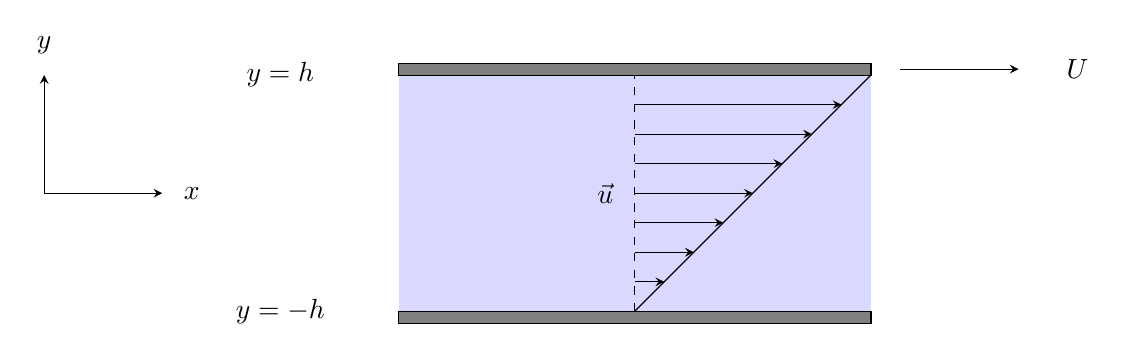
\begin{tikzpicture}[scale=1.5]
		% fluid
		\path[fill=blue!15!] (0,0) rectangle (4,2);
		
		% plates
		\draw[fill=gray] (0,0) rectangle (4,-0.1);
		\draw[fill=gray] (0,2) rectangle (4,2.1);
		
		% plate heights
		\node at (-1,0) {$y=-h$};
		\node at (-1,2) {$y=h$};
		
		% top plate velocity
		\draw[->, >=stealth] (4.25,2.05) -- (5.25,2.05);
		\node at (5.75,2.05) {$U$};
		
		% reference frame
		\draw[<->, >=stealth] (-3,2) -- (-3,1) -- (-2,1);
		\node at (-3,2.25) {$y$};
		\node at (-1.75,1) {$x$};
		
		% velocity field (jonathan's figure)
		\node at (1.75,1) {$\vec{u}$};
		\draw[dashed] (2,0) -- (2,2);
		\draw (2,0) -- (4,2);
		\foreach \x in {0.25,0.5,...,1.75}{
		    \draw[->, >=stealth] (2,\x) -- (2+\x,\x);
		}
	\end{tikzpicture}
	\caption{A schematic of the Couette flow configuration, with the velocity profile included.}
\end{figure}

\begin{figure}[H]
    \centering
    \includegraphics[scale=0.75]{figures/couette_velocity-profile.pdf}
    \caption{A plot of the velocity profile for Couette flow for $U = 0.1, 1, 10$ m/s}
\end{figure}